\documentclass[10pt, xcolor=table]{beamer}

\usetheme{Warsaw}
%%%%%\usecolortheme{crane}
%%%%%\usecolortheme{orchid}
% \usecolortheme{orchid}
\definecolor{azull}{rgb}{.10,.20,.3}
\usecolortheme[named=azull]{structure}
\usefonttheme{structurebold}
%\usefonttheme{professionalfonts}
\useinnertheme{rounded}
\newcommand{\maggen}{\textbf{magGen}}
\usepackage[spanish]{babel}% división de silabas en spanish
\usepackage[utf8]{inputenc}
\usepackage{amsmath}
\usepackage{multirow}
\usepackage[table]{xcolor}
%\usepackage{amsfonts}
%\usepackage{amssymb}
%\usepackage{stmaryrd}
\usepackage{graphicx}
%\usepackage[all]{xy}
\usepackage{listings}
\definecolor{lbcolor}{rgb}{0.9,0.9,0.9}
\definecolor{gris}{RGB}{124,129,140}
\definecolor{azul}{rgb}{0.0,0.3,0.6}

\newcommand{\textbtt}[1]{\texttt{\textbf{#1}}}

\lstset{
    backgroundcolor=\color{lbcolor},
    tabsize=2,
    rulesepcolor=\color{azul},
    language=C++,
    morekeywords={repeat, until, procedure, then, from,
                  lexeme_d, as_lower_d, longest_d,
                  \!, \+, \*, \>\>, \-, \&, \|, \=, \%,
                  anychar_p, alnum_p, alpha_p, digit_p, lower_p, upper_p, space_p, ch_p, str_p, oct_p, hex_p, uint_p, int_p, real_p, eps_p, end_p,
                  symbols, add,
                  end},
    basicstyle=\tiny,
    aboveskip={1\baselineskip},
    columns=[c]fixed,
    showstringspaces=false,
    extendedchars=true,
    breaklines=true,
    prebreak = \raisebox{0ex}[0ex][0ex]{\ensuremath{\hookleftarrow}},
    frame=single,
    showtabs=false,
    showspaces=false,
    showstringspaces=false,
    identifierstyle=\ttfamily,
    keywordstyle=\color[rgb]{0.1,0.1,0.6}\bfseries,
    commentstyle=\color[rgb]{0.133,0.545,0.133},
    stringstyle=\color[rgb]{0.627,0.126,0.941},
    keepspaces=true,
    escapeinside=``,
    numbersep=5pt,
    numberstyle=\scriptsize
}

\lstdefinelanguage{specmag}{
  keywords={compute, end, all, semantic, domain, attributes, rules, sort, op, function, infix, prefix, postfix, syn, inh, left, right, non_assoc, and, and_eq, asm, auto, bitand, bitor, break, case, catch, class, compl, const, const_cast, continue, default, delete, do, double, dynamic_cast, else, enum, explicit, export, extern, false, for, friend, goto, if, inline, long, mutable, namespace, new, not, not_eq, operator, or, or_eq, private, protected, public, register, reinterpret_cast, return, short, signed, sizeof, static, static_cast, struct, switch, template, this, throw, true, try, typedef, typeid, typename, union, unsigned, using, virtual, void, volatile, wchar_t, while, xor, xor_eq, bool, char, float, int, string
%   ,repeat, until, procedure, then, from
  ,cout, endl
  },
  sensitive=true,
  morecomment=[s]{/*}{*/},
  morecomment=[l]{\//},
  morestring=[d]{"}
}

\newcommand{\urllink}[1]{\htmladdnormallink{#1}{#1}}
\definecolor{linkcol}{rgb}{0,0,0.4} 
\definecolor{citecol}{rgb}{0.5,0,0} 
\setbeamercovered{transparent=5}

\subtitle[Generador de Evaluadores Estáticos para MAG]{Generador de Evaluadores Estáticos para MAG}
\title[Generador de Evaluadores Estáticos para MAG]{\maggen}
%\subtitle{Abstracci\'on: Acciones y Funciones}
\author{Gerardo Luis Kilmurray - Gonzalo Martín Picco}
\institute[U.N.R.C.]{
    Departamento de Computaci\'on\\
    Facultad de Ciencias Exactas, F\'isico-Qu\'imicas y Naturales\\
    Universidad Nacional de R\'io Cuarto}
% \date{Marzo de 2010}

\begin{document}

\frame{\titlepage}

\frame{
    \frametitle{Temario:}
    \tableofcontents
}

\section{\textquestiondown Qué es magGen?}

\frame{
\frametitle{\textquestiondown Qué es \maggen?}
    \begin{block}{}
        \maggen\ es una herramienta generadora de evaluadores estáticos para la familia MAG. 
    \end{block}
    \pause

    \begin{center}
        {\huge \textbf{mag} + \textbf{Gen}}\\
        \textit{Multi-plans Attribute Grammar} - \textit{Generator}
    \end{center}
    \pause

    Características distinguibles:
    \begin{itemize}
        \item Basa su funcionamiento en gramática MAG.
        \item Generación de mínima cantidad de planes.
        \item Generación de Evaluadores estáticos.
    \end{itemize}
}

\subsection{Motivación}
\frame{
    \frametitle{Motivación}
    
    \begin{block}{}
        En las ciencias de la computación los lenguajes juegan un rol muy importante en muchas disciplinas. Desde los comienzos se buscaron \textit{mecanismos} para describirlos y manejarlos.
    \end{block}
    \pause
    
    \begin{block}{}
        D. Knuth introdujo en 1966 las \textbf{gramáticas de atributos} (GA), estas se han utilizado ampliamente para el desarrollo de herramientas de procesamiento de lenguajes formales y, además, para especificar la semántica de lenguajes de programación.
    \end{block}
    \pause
    
    \begin{block}{}
        En 1998, Wuu Yang caracteriza una nueva familia denominada \textbf{Gramática de Atributos Multi-planes}. 
    \end{block}
    \pause
    
    \begin{center}
        {\large\textbf{Al momento no existían herramientas basadas en esta familia de Gramáticas de Atributos}}
    \end{center} 
}

\section{Preliminares}

\frame{
    \frametitle{Notación}
    \begin{block}{Gramática de atributos (Informal)}
        En una \textbf{Gramática de Atributos} (GA), se relaciona cada símbolo de una \textit{Gramática Libre de Contexto} con un conjunto de atributos. Cada regla o producción tiene asociado un \textit{conjunto de reglas semánticas}, denominadas también \textit{ecuaciones}.
    \end{block}
    \pause

    \textbf{Instancia:} Ocurrencia de un símbolo de la gramática asociado a un atributo. 
}

\begin{frame}[fragile]
    \frametitle{Ejemplo GA}

\begin{figure}[h]
\begin{center}
\begin{tabular}{c}
\begin{lstlisting}[backgroundcolor=\color{white}, basicstyle=\scriptsize, language=, linewidth=7.5cm]
(R1)    S `$\rightarrow$` XYZ      
            S.s0 := X.s1 + Y.s2 + Y.s3 + Z.s4
            X.i1 := Y.s3  
            Y.i2 := X.s1
            Y.i3 := Y.s2
(R2)    Y `$\rightarrow$` m        
            Y.s2 := Y.i2
            Y.s3 := 1
(R3)    Y `$\rightarrow$` n        
            Y.s2 := 2
            Y.s3 := Y.i3
(R4)    X `$\rightarrow$` m        
            X.s1 := X.i1
(R5)    Z `$\rightarrow$` Y        
            Z.s4 := Y.s3
            Y.i2 := 3
            Y.i3 := Y.s2
\end{lstlisting} 
\end{tabular}
\end{center}
\end{figure}

    \pause
    \vspace{-0.5cm}
    \begin{block}{Ejemplo de instancia}
        Y.i3 $\Leftrightarrow$ Ocurrencia del símbolo $Y$ asociado al atributo $i3$.
    \end{block}
\end{frame}

\subsection{Gramáticas de Atributos Multiplanes (MAG)}

\frame{
    \frametitle{Gramáticas de Atributos Multiplanes}

    \begin{block}{Dependencias directas de una producción}
        Se denota como \textbf{DP(p)}	
        $$
          DP(p) = \{(X_{i}.a, X_{j}.b) | X_{i}.a \rightarrow Y_{j}.b \in R^{p} \}
        $$
    \end{block}
    \pause
    
    Dado un símbolo X de una gramática de atributos

    $$\textbf{Down(X)} =  \{(a,b) | a \rightarrow b \} con\ a,b \in A(X)\}$$
}

\frame{
    \frametitle{Gramáticas de Atributos Multiplanes (cont.)}

    \begin{block}{Conjunto de dependencias aumentadas}
        Sea $q$ una producción de la forma $X_{0}\rightarrow \alpha_{0} X_{1} \alpha_{1} X_{2} \dots X_{k} \alpha_{k}$. Sea $p_{i}$ una producción cuya parte izquierda es $X_{i}$ ($1\leqslant i \leqslant k$). 
        $$
        ADP (q | p_{1}, p_{2}, \dots, p_{k}) = DP(q) \bigcup\limits_{k}^{i=1}{DGC_{X_{i}}} (p_{i})
        $$
        se denota como $\textbf{ADP (q $|$ p}_{\textbf{1}}\textbf{, p}_{\textbf{2}}\textbf{, \dots , p}_{\textbf{k}}\textbf{)} $
    \end{block}
    \pause
    
    $\textbf{DCG}_{\textbf{X}}\textbf{(p)}$ contiene las dependencias, entre las instancias de la gramática, para el símbolo \texttt{X}, acotando el análisis para la producción \textit{p} y los posibles contextos inferiores.
    $$
    \bigcup\limits_{\textit{todo p}}{DCG_{X} (p) = Down (X)}
    $$
}

\frame{
    \frametitle{Gramáticas de Atributos Multiplanes (cont.)}

    El conjunto de todas las posibles dependencias aumentadas para una producción \textbtt{q} se define como:
    $$
    SADP(q) = \bigcup\limits_{q\in P}{ADP (q | p_{1}, p_{2}, \dots, p_{k})} 
    $$
    \pause

    \begin{exampleblock}{Gramática de Atributos Multiplanes (MAG)}
        Una gramática \textit{G} es una \textit{Gramática de Atributos Multiplanes} si y solo si 
        $$
        \forall q : q \in P: (\forall g:g\ es\ un\ grafo\ de\ q \wedge g \in SADP(q) : g\ es\ no\ circular) 
        $$
    \end{exampleblock}
}

\frame{
    \frametitle{Familias de gramáticas de atributos}

    \begin{center}
        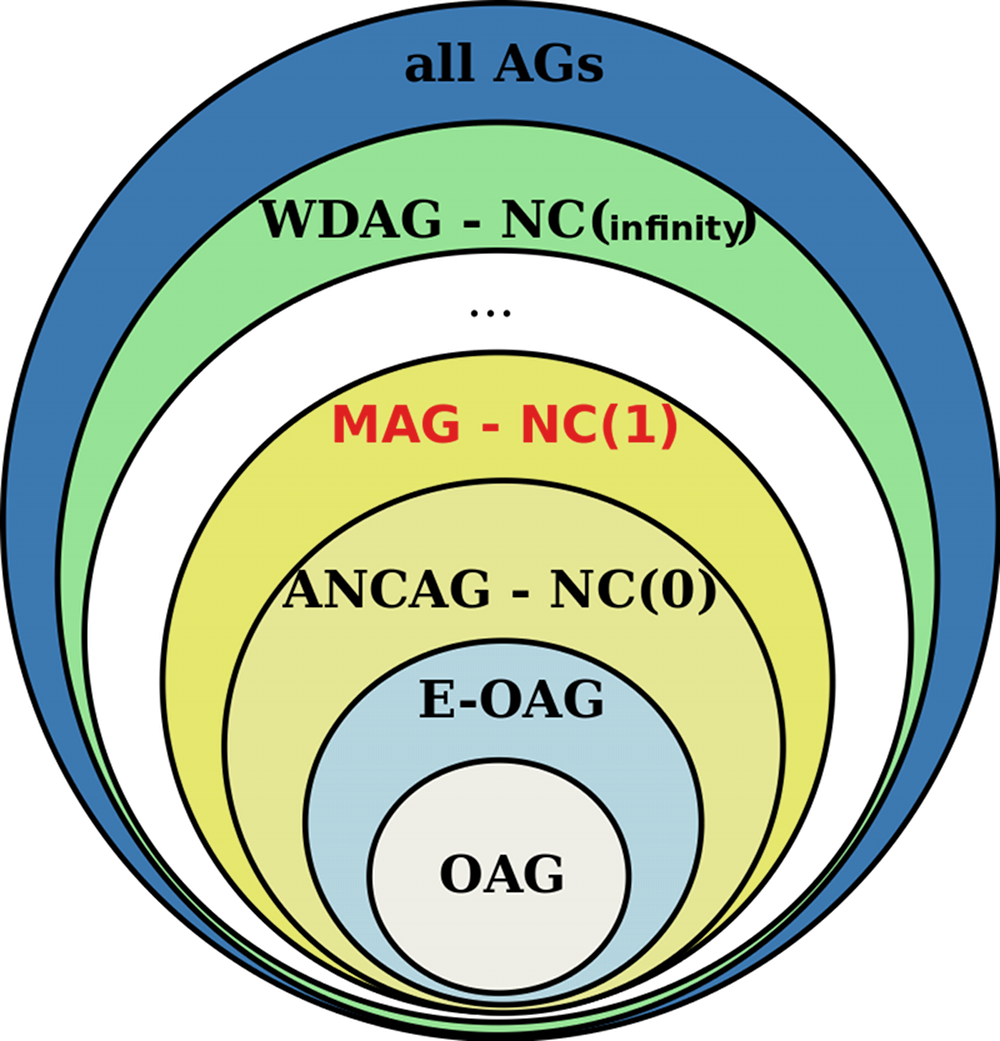
\includegraphics[width=192px, height=200px]{./familias_ag.png}
    \end{center}
}

\subsection{Evaluador estático}

\frame{
    \frametitle{Evaluador estático}
    
    \begin{block}{}
	Los métodos estáticos deben tener en cuenta todos los árboles sintácticos posibles a ser generados por la gramática y calcular las dependencias, entre las instancias de los atributos, para cada uno de ellos. 
    \end{block}
    \pause

    \begin{block}{Contexto de una producción}
        Tres tipos de dependencias definen el \textit{contexto} de una producción:

        \begin{itemize}
            \item Directas obtenidas por las ecuaciones de $p$.
            \item Impuestas por el contexto superior.
            \item Impuestas en el contexto inferior.
        \end{itemize}
    \end{block}
    \pause

    Instancias diferentes de una producción $p$ tendrán las mismas dependencias directas, pero podrán tener diferentes dependencias impuestas por los contextos inferiores y superiores. 
}

\subsection{Planes de evaluación}

\frame{
    \frametitle{Planes de evaluación}

    \begin{block}{}
        Luego del análisis de las dependencias, los grafos ADP acícliclos inducen un orden entre las ecuaciones que deben computarse.
    \end{block}
    \pause

    \begin{block}{}
        El proceso de construcción de planes, considera el tres factores:
            \begin{itemize}
                \item Orden inducido por las dependencias.
                \item Orden superior para la evaluación de las instancias.
                \item El contexto de aplicación.
            \end{itemize}
     \end{block}
    \pause

    \begin{block}{Plan de Evaluación}
    	Un plan de evaluación esta dado por un orden consistente con las dependencias para la computación de las ecuaciones que definen a cada instancia de la gramática.
    \end{block}
}

\subsection{Secuencias de visitas}
\frame{
    \frametitle{Secuencia de Visita}
	
    \begin{block}{}
	El concepto de \emph{Secuencias de Visita} fue presentado en 1980, por \textbf{Uwe Kastens}  como un método de evaluación polinomial para la familia $OAG$.
    \end{block}
    \pause
	
	\begin{block}{}
        Su funcionamiento se basa en la visita de los nodos de los árboles de derivación para lograr la evaluación del árbol. Este método se apoya en los planes de evaluación de la gramática.
    \end{block}
    \pause
    
    \begin{exampleblock}{}
        Los evaluadores basados en secuencias de visita pertenecen a una familia denominada \textbf{Evaluadores Multivisita}, ya que el proceso de evaluación puede requerir múltiples visitas a cada nodo para evaluarlo.
    \end{exampleblock}
}

\frame{
    \frametitle{Secuencia de Visita (cont.)}

    \begin{block}{Definición}
    	Sea $n$ un nodo de un árbol atribuido $T$. Una secuencia de visita en el nodo $n$ \textbf{es una secuencia de tres operaciones o acciones}: 
    	\emph{visit(child,i)}, \emph{compute(at)} y \emph{leave(i)}.
    \end{block}
    \pause

    \begin{description}
    	\item [visit(child,i)] indica que el evaluador debe moverse (visitar) el nodo hijo \emph{child} de $n$ y corresponde a la \emph{i-ésima} visita al nodo hijo.
	\pause

    	\item [compute(at)] indica que debe evaluarse la ecuación que define $at$ en la producción $p$ aplicada correspondiente al nodo $n$.
	\pause

    	\item[leave(i)] indica que ha finalizado la visita \emph{i-ésima} en el nodo corriente y que se debe visitar al nodo padre.
    \end{description}
}

\section{magGen}
\subsection{Herramientas}
\frame{
    \frametitle{\maggen: Herramientas usadas}

    \begin{tabular}{p{4.5cm}p{6.5cm}}
    \begin{itemize}
	    \item C++%\footnote{http://public.research.att.com/~bs/C++.html}.
		\item Boost C++ Libraries%\footnote{http://www.boost.org/}.
		    \begin{itemize}
			\item Spirit Parser Framework%\footnote{http://boost-spirit.com/home/}.
			\item The Boost Graph Library (BGL)%\footnote{http://www.boost.org/doc/libs/release/libs/graph/}.
		    \end{itemize}
		\item GraphViz% \footnote{http://www.graphviz.org/}.
        \item Eclipse
		\item Subversion
		\item \LaTeXe
	\end{itemize}&
	\begin{itemize}
		\item kile 
		\item Nemiver + gbd
		\item Dia
		\item Bouml
		\item Cmake
		\item Análisis estático de código:
		\begin{itemize}
			\item CCCC
			\item gcov
		\end{itemize}
	\end{itemize}\\
	\end{tabular}
}

\subsection{Funcionamiento}

\frame{
    \frametitle{\maggen: Funcionamiento}
    
    El funcionamiento de \maggen\ esta dado por la integración de 4 etapas, consideradas principales, que marcaron el proceso de desarrollo de la herramienta:
    \begin{itemize}
        \item Lenguaje especificación de MAG.
	\pause
        \item Parser del lenguaje,representación interna y chequeos.
	\pause
        \item Construcción de grafos y aplicación de algoritmos de cómputo de planes y secuencias de visita.
	\pause
        \item Generación de código.
    \end{itemize}
    \pause

    El cómputo de \maggen\ se realiza atravesando cada una de estas etapas secuencialmente, es decir, la terminación exitosa de una, habilita la siguiente; por lo tanto cada etapa mantiene su salida de errores de manera independiente. 
}

\begin{frame}[fragile]
    \frametitle{\maggen: Funcionamiento (cont.)}

    La salida normal de \maggen\ que indica que se han realizado todas las etapas correctamente, es la siguiente:

\begin{figure}[h]
\begin{center}
\begin{tabular}{c}
\begin{lstlisting}[backgroundcolor=\color{white}, basicstyle=\footnotesize, language=, linewidth=8cm]
* Parsing grammar ---------- [  OK  ]
* Generate graphs ---------- [  OK  ]
* Build plans -------------- [  OK  ]
* Build visit sequence ----- [  OK  ]
* Generation code ---------- [  OK  ]

Generation complete in: 0.372814 seconds.
\end{lstlisting}
\end{tabular}
\end{center}
\end{figure}
\end{frame}

\frame{
    \frametitle{Arquitectura}
    
    \begin{center}
        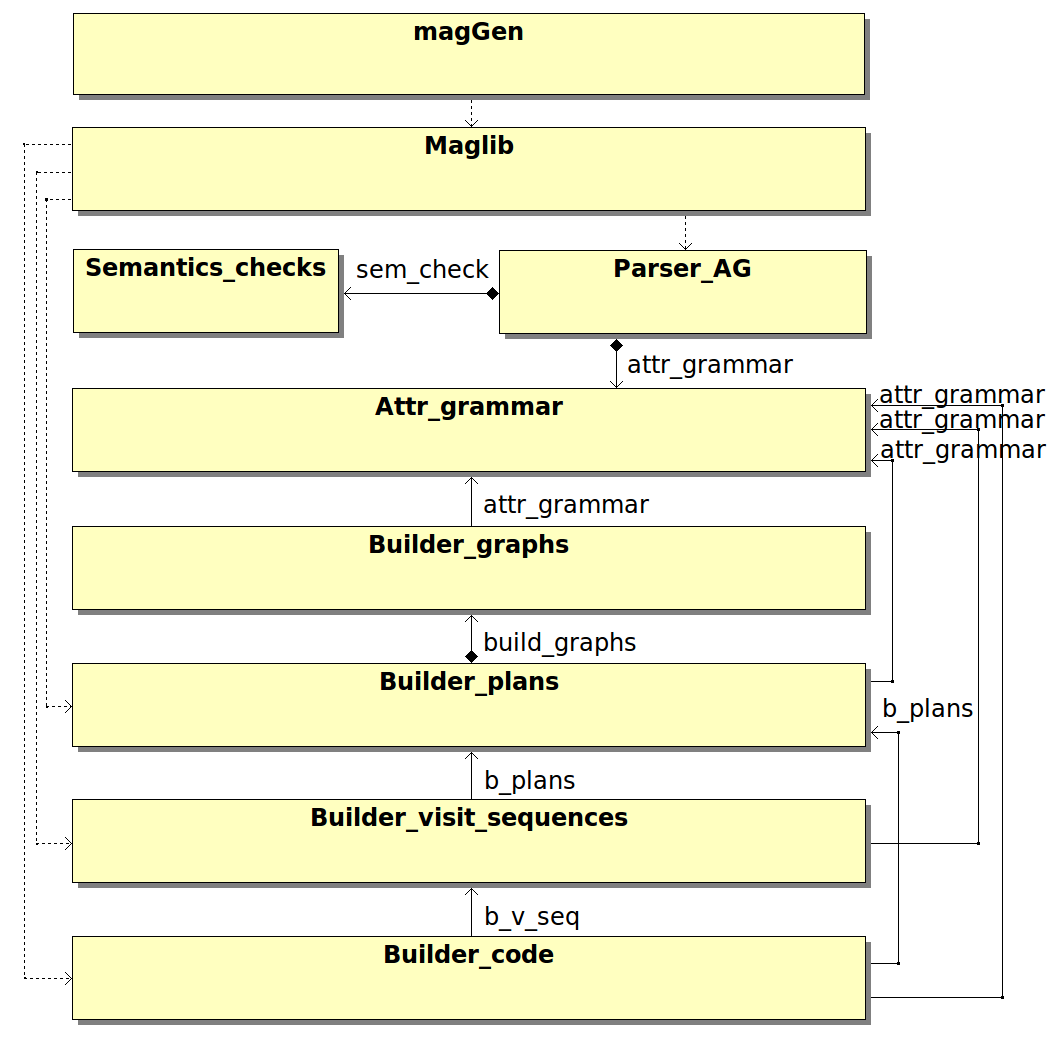
\includegraphics[width=204px, height=200px]{./arquitectura.png}
    \end{center}
}

\subsection{Lenguaje de Especificación}
\begin{frame}[fragile]
    \frametitle{Lenguaje especificación de MAG}

    \begin{block}{Especificación}
    La secciones que conforman la descripción de una MAG, se corresponden con las características de una gramática en esta familia.
    \end{block}
    
\begin{figure}[h]
\begin{center}
\begin{tabular}{c}
 \begin{lstlisting}[language=specmag, basicstyle=\small, linewidth=7cm]
    semantic domain
            <sorts>
            <operators>
            <functions>
    attributes
            <attrs>
    rules
            <rule0>
                    <equations>
            `$\ldots$`
            <ruleN>
                    <equations>
\end{lstlisting} 
\end{tabular}
\end{center}
\end{figure}
\end{frame}

\begin{frame}[fragile]
\frametitle{Gramática MAG presentada por Wuu Yang}

\begin{figure}[h]
\begin{center}
\begin{tabular}{c}
\begin{lstlisting}[basicstyle=\scriptsize, language=, linewidth=7.5cm]
(R1)    S `$\rightarrow$` XYZ      
            S.s0 := X.s1 + Y.s2 + Y.s3 + Z.s4
            X.i1 := Y.s3  
            Y.i2 := X.s1
            Y.i3 := Y.s2
(R2)    Y `$\rightarrow$` m        
            Y.s2 := Y.i2
            Y.s3 := 1
(R3)    Y `$\rightarrow$` n        
            Y.s2 := 2
            Y.s3 := Y.i3
(R4)    X `$\rightarrow$` m        
            X.s1 := X.i1
(R5)    Z `$\rightarrow$` Y        
            Z.s4 := Y.s3
            Y.i2 := 3
            Y.i3 := Y.s2
\end{lstlisting} 
\end{tabular}
\end{center}
\end{figure}
\end{frame}

\begin{frame}[fragile]
\frametitle{Especificación en lenguaje de \maggen}

\begin{lstlisting}[basicstyle=\scriptsize, language=specmag, linewidth=10cm]
semantic domain
    op infix  (10, left) +: int, int -> int;

attributes
    s0: syn <int> of {S};
    s1: syn <int> of {X};
    s2: syn <int> of {Y};
    s3: syn <int> of {Y};
    s4: syn <int> of {Z};
    i1: inh <int> of {X};
    i2: inh <int> of {Y};
    i3: inh <int> of {Y};

rules
    S ::= X Y Z
        compute
            S[0].s0 = X[0].s1 + Y[0].s2 + Y[0].s3 + Z[0].s4;
            X[0].i1 = Y[0].s3;
            Y[0].i2 = X[0].s1;
            Y[0].i3 = Y[0].s2;
        end;
\end{lstlisting}
\end{frame}

\begin{frame}[fragile]
\frametitle{Especificación en lenguaje de \maggen\ (cont.)}

\begin{lstlisting}[basicstyle=\scriptsize, language=specmag, linewidth=10cm]
    Y ::= 'm'
        compute
            Y[0].s2 = Y[0].i2;
            Y[0].s3 = 1;
        end;
    Y ::= 'n'
        compute
            Y[0].s2 = 2;
            Y[0].s3 = Y[0].i3;
        end;
    X ::= 'm'
        compute
            X[0].s1 = X[0].i1;
        end;
    Z ::= Y
        compute
            Z[0].s4 = Y[0].s3;
            Y[0].i2 = 3;
            Y[0].i3 = Y[0].s2;
        end;


\end{lstlisting}

\end{frame}

\frame{
    \frametitle{\maggen: Chequeos}

    Sobre la MAG de entrada se verifican:
    \begin{itemize}
        \item Precedencia y Asociatividad de operadores dentro de expresiones.
	\pause
	\item Alcanzabilidad de símbolos y reglas.
	\pause
        \item Consistencia de bloque de atributos y bloque de reglas.
	\pause
        \item Gramática bien definida
	\pause
        \begin{itemize}
            \item Atributos sintetizados del símbolo de la parte izquierda.
	    \pause
            \item Atributos heredados de símbolos de la parte derecha.
	    \pause
            \item Ecuaciones sólo de los atributos de los símbolos de la regla.
	    \pause
            \item Inexistencia de ecuaciones para atributos heredados del símbolo de la izquierda y para atributos sintetizados de símbolos de la parte derecha.
	    \pause
            \item Múltiples ecuaciones para un atributo.
	    \pause
            \item Consistencia de los índices de las instancias que aparecen en las ecuaciones.
	    \pause
            \item Condiciones de una gramática extendida.
        \end{itemize}
    \end{itemize}
}
\subsection{Builders}
\frame{
    \frametitle{\maggen: Generate graphs}
    
    Luego de los chequeos semánticos sobre la gramática de entrada, se construyen los siguientes grafos:
    \pause
    \begin{itemize}
	\item Grafos \textbf{DP}: Dependencias directas de cada producción.
	\pause
	\item Grafos \textbf{Down}: Dependencias entre atributos de cada símbolo.
	\pause
	\item Grafos \textbf{DCG}: Dependencias entre atributos de cada símbolos acotado a una producción.
	\pause
	\item Grafos \textbf{ADP}: Grafos de dependencias aumentadas.
    \end{itemize}
    \pause

    \begin{block}{}
	La construcción de los grafos permite realizar chequeos de ciclicidad y servir de base (grafos ADP) para la construcción de planes de evaluación.
    \end{block}
}

\begin{frame}[fragile]
    \frametitle{magGen - Grafo DP}

\begin{figure}[h]
\begin{center}
\begin{tabular}{c}
\begin{lstlisting}[basicstyle=\scriptsize, language=, linewidth=7.5cm]
(R1)    S `$\rightarrow$` XYZ
            S.s0 := X.s1 + Y.s2 + Y.s3 + Z.s4
            X.i1 := Y.s3  
            Y.i2 := X.s1
            Y.i3 := Y.s2
\end{lstlisting}
\end{tabular}
\end{center}
\end{figure}

\begin{center}
    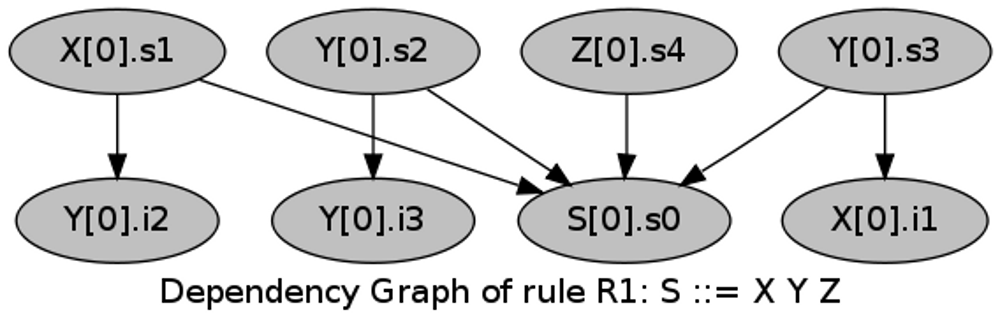
\includegraphics[width=175px, height=58px]{./1_dp_graph.png}
\end{center}

\end{frame}

\begin{frame}[fragile]
    \frametitle{magGen - Grafo Down}

\begin{tabular}{c c}
\begin{lstlisting}[basicstyle=\scriptsize, language=, linewidth=7cm]
(R1) S `$\rightarrow$` XYZ
       S.s0 := X.s1 + Y.s2 + Y.s3 + Z.s4
       X.i1 := Y.s3
       Y.i2 := X.s1
       Y.i3 := Y.s2
(R2) Y `$\rightarrow$` m
       Y.s2 := Y.i2
       Y.s3 := 1
(R3) Y `$\rightarrow$` n
       Y.s2 := 2
       Y.s3 := Y.i3
(R4) X `$\rightarrow$` m
       X.s1 := X.i1
(R5) Z `$\rightarrow$` Y
       Z.s4 := Y.s3
       Y.i2 := 3
       Y.i3 := Y.s2
\end{lstlisting}
& \hspace{1cm}\parbox[c]{1em}{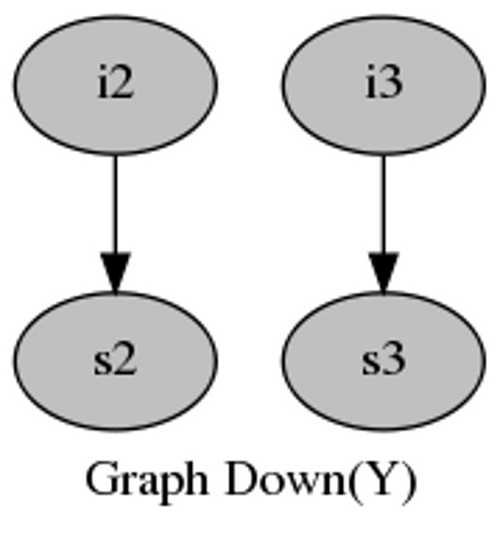
\includegraphics[width=75px, height=82px]{./8_down_graph.png}}\\
\end{tabular}

\end{frame}

\begin{frame}[fragile]
    \frametitle{magGen - Grafo Down}

\begin{tabular}{c c}
\begin{lstlisting}[basicstyle=\scriptsize, language=, linewidth=7cm]
(R1) S `$\rightarrow$` XYZ
       S.s0 := X.s1 + Y.s2 + Y.s3 + Z.s4
       X.i1 := Y.s3
       Y.i2 := X.s1
       Y.i3 := Y.s2
(R2) Y `$\rightarrow$` m
       Y.s2 := Y.i2
       Y.s3 := 1
(R3) Y `$\rightarrow$` n
       Y.s2 := 2
       Y.s3 := Y.i3
(R4) X `$\rightarrow$` m
       X.s1 := X.i1
(R5) Z `$\rightarrow$` Y
       Z.s4 := Y.s3
       Y.i2 := 3
       Y.i3 := Y.s2
\end{lstlisting}
& \hspace{1cm}\parbox[c]{1em}{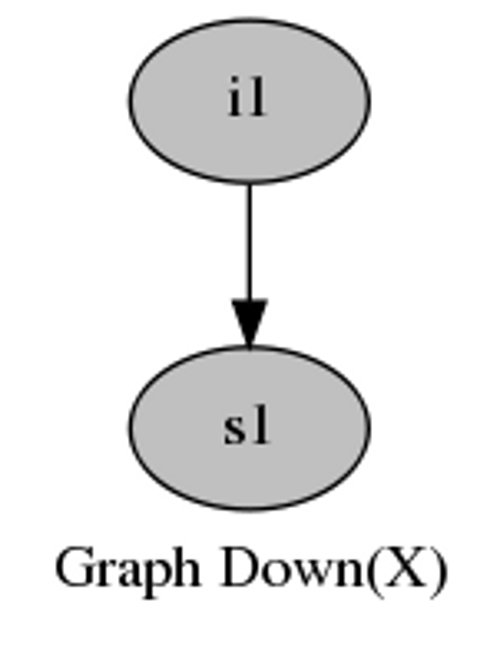
\includegraphics[width=75px, height=82px]{./7_down_graph.png}}\\
\end{tabular}

\end{frame}

\begin{frame}[fragile]
    \frametitle{magGen - Grafo DCG}
\begin{center}        
\begin{tabular}{p{6cm}}
\begin{lstlisting}[basicstyle=\scriptsize, language=, linewidth=7cm]
...
(R2) Y `$\rightarrow$` m
       Y.s2 := Y.i2
       Y.s3 := 1
(R3) Y `$\rightarrow$` n
       Y.s2 := 2
       Y.s3 := Y.i3
...
\end{lstlisting}
\end{tabular}
\end{center}
\begin{center}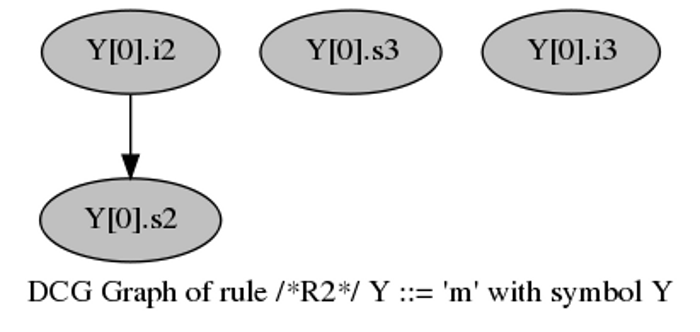
\includegraphics[width=160px, height=76px]{./11_dcg_graph.png}\end{center}
\end{frame}

\begin{frame}[fragile]
    \frametitle{magGen - Grafo DCG}
\begin{center}        
\begin{tabular}{p{6cm}}
\begin{lstlisting}[basicstyle=\scriptsize, language=, linewidth=7cm]
...
(R2) Y `$\rightarrow$` m
       Y.s2 := Y.i2
       Y.s3 := 1
(R3) Y `$\rightarrow$` n
       Y.s2 := 2
       Y.s3 := Y.i3
...
\end{lstlisting}
\end{tabular}
\end{center}
\begin{center}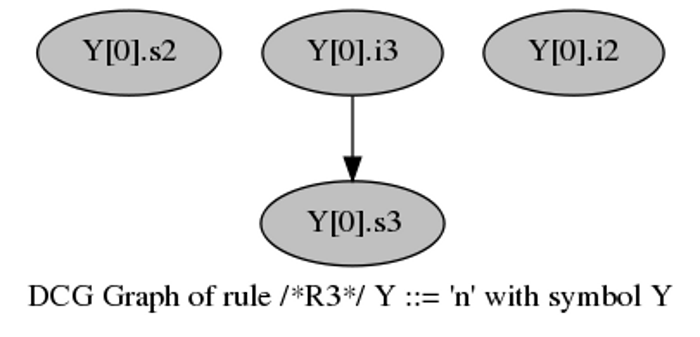
\includegraphics[width=160px, height=77px]{./12_dcg_graph.png}\end{center}
\end{frame}

\begin{frame}[fragile]
    \frametitle{magGen - Grafo ADP}

\begin{tabular}{c p{4.5cm}}
\hspace{-0.5cm}\begin{lstlisting}[basicstyle=\scriptsize, language=, linewidth=6.6cm]
(R1) S `$\rightarrow$` XYZ
       S.s0 := X.s1 + Y.s2 + Y.s3 + Z.s4
       X.i1 := Y.s3
       Y.i2 := X.s1
       Y.i3 := Y.s2
(R2) Y `$\rightarrow$` m
       Y.s2 := Y.i2
       Y.s3 := 1
(R3) Y `$\rightarrow$` n
       Y.s2 := 2
       Y.s3 := Y.i3
(R4) X `$\rightarrow$` m
       X.s1 := X.i1
(R5) Z `$\rightarrow$` Y
       Z.s4 := Y.s3
       Y.i2 := 3
       Y.i3 := Y.s2
\end{lstlisting}
&\hspace{0.2cm}\parbox[c]{1em}{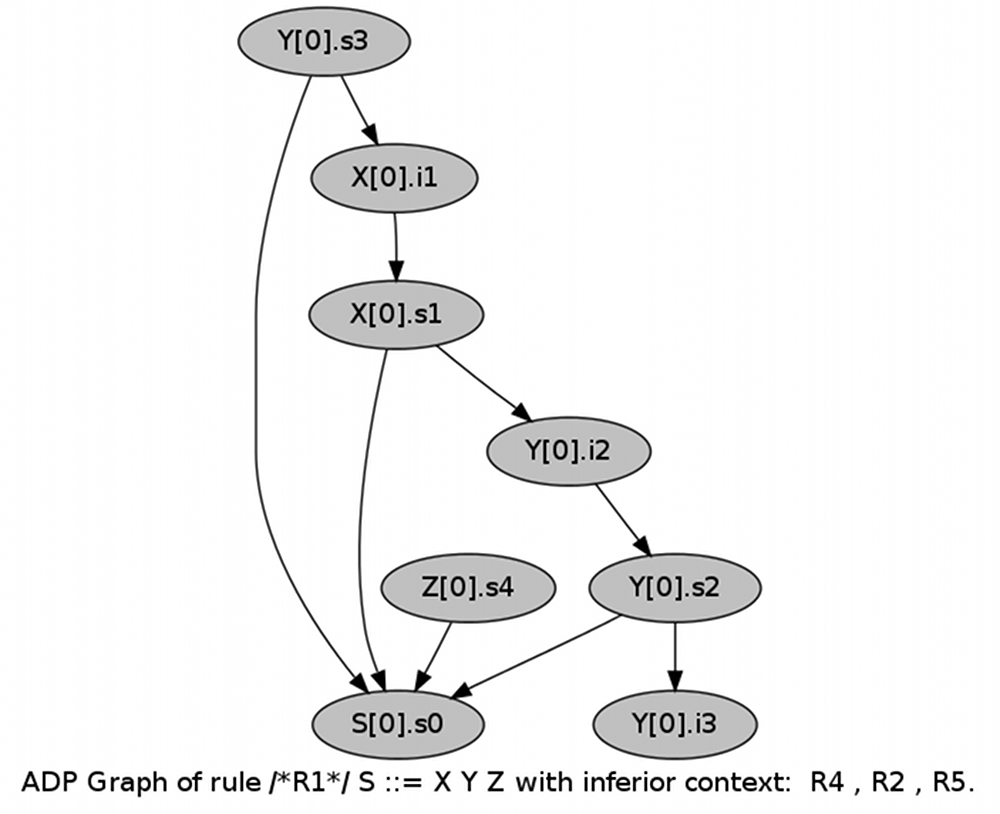
\includegraphics[width=149px, height=150px]{./15_adp_graph.png}}
\end{tabular}

\end{frame}

\begin{frame}[fragile]
    \frametitle{magGen - Grafo ADP}
\begin{tabular}{c p{4.5cm}}
\hspace{-0.5cm}\begin{lstlisting}[basicstyle=\scriptsize, language=, linewidth=6.6cm]
(R1) S `$\rightarrow$` XYZ
       S.s0 := X.s1 + Y.s2 + Y.s3 + Z.s4
       X.i1 := Y.s3
       Y.i2 := X.s1
       Y.i3 := Y.s2
(R2) Y `$\rightarrow$` m
       Y.s2 := Y.i2
       Y.s3 := 1
(R3) Y `$\rightarrow$` n
       Y.s2 := 2
       Y.s3 := Y.i3
(R4) X `$\rightarrow$` m
       X.s1 := X.i1
(R5) Z `$\rightarrow$` Y
       Z.s4 := Y.s3
       Y.i2 := 3
       Y.i3 := Y.s2
\end{lstlisting}
&\hspace{0.2cm}\parbox[c]{1em}{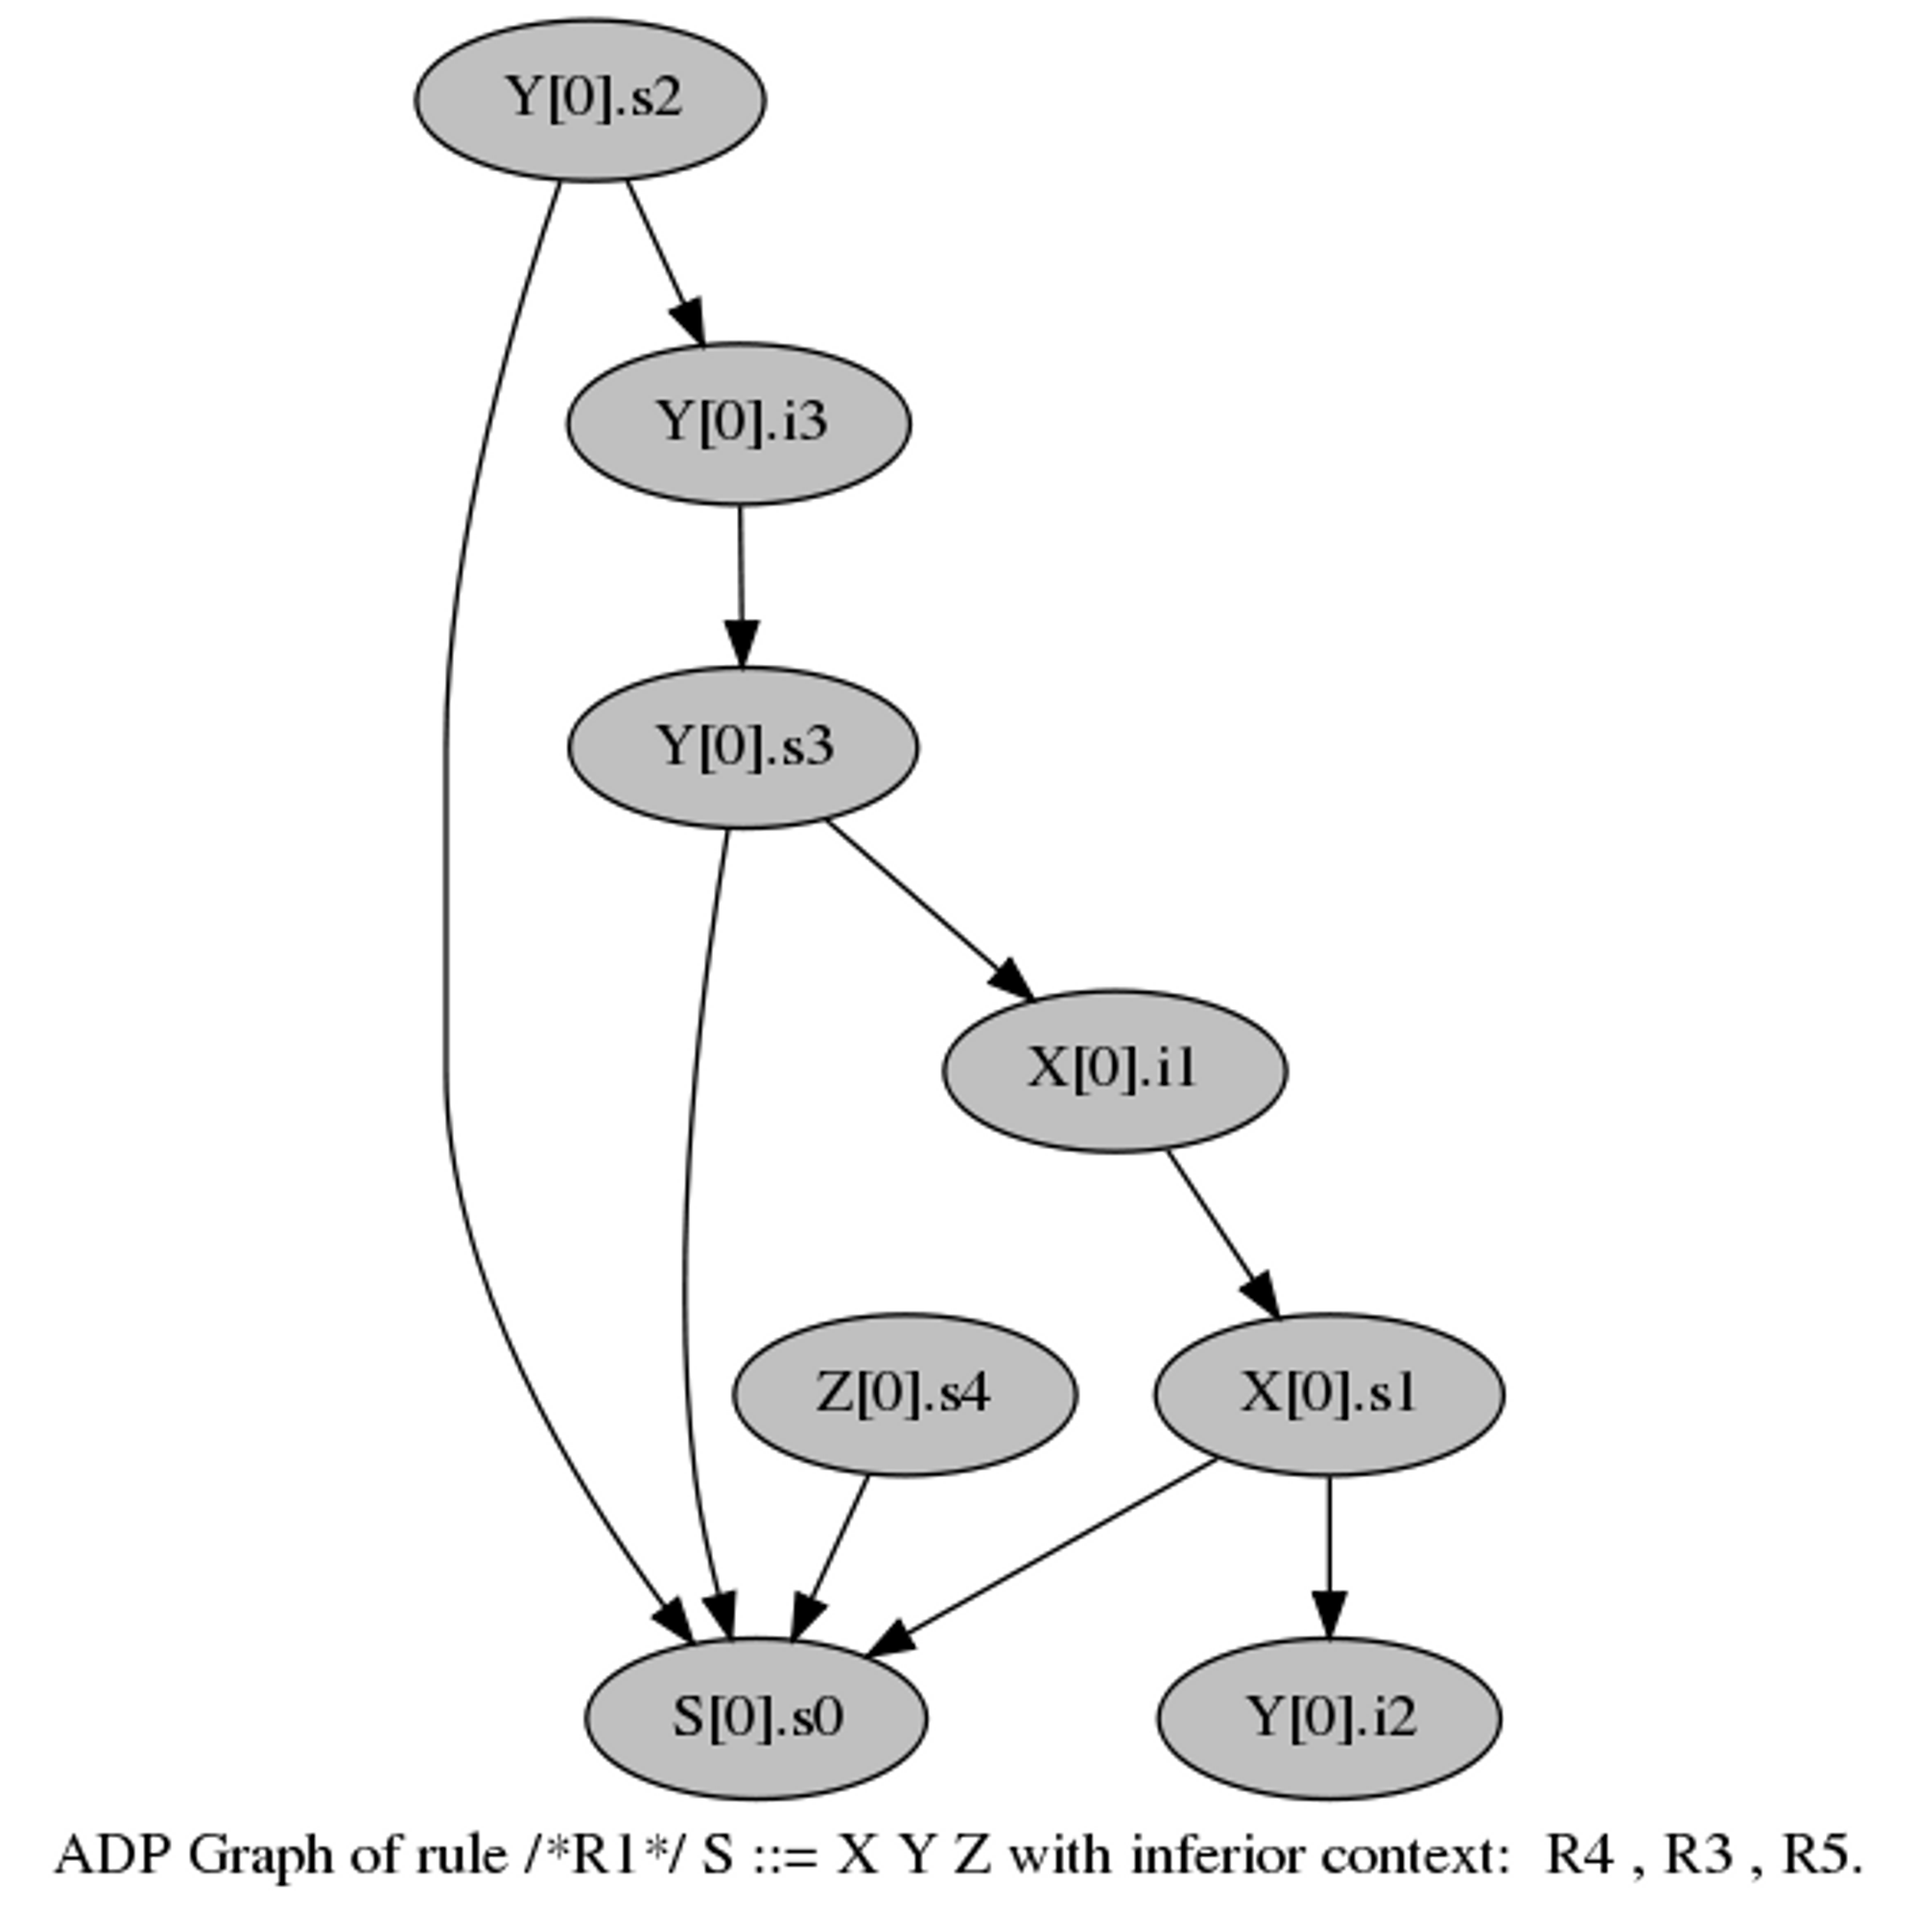
\includegraphics[width=149px, height=150px]{./16_adp_graph.png}}
\end{tabular}

\end{frame}

\begin{frame}[fragile]
    \frametitle{Ciclicidad}

    \begin{block}{}
	\begin{itemize}
	    \item El chequeo de ciclicidad es realiza sobre los grafos ADP.
	    \pause
	    \item Esta basado en el algoritmo de búsqueda en profundidad (Depth-first search) de \textbf{boost} combinado con la creación de un ``visitador'' especializado.
	    \pause
	    \item El subgrafo es mostrado al usuario en caso de detección de ciclo, sino es descartado.
	\end{itemize}
    \end{block}
    \pause

La salida de \maggen\ cuando se detecta ciclicidad, es:

\begin{lstlisting}[backgroundcolor=\color{white}, basicstyle=\footnotesize, language=] 
   * Parsing grammar ---------- [  OK  ]
   * Generate graphs ---------- [  OK  ]
   * Build plans -------------- [ ABORT ]

   ERROR: One o more graph ADP has an cycle in its dependencies. Look the folder ./out_maggen/graphs/CYCLIC_graphs/ for more details.
\end{lstlisting}
\end{frame}

\frame{
    \frametitle{\maggen - Plan de evaluacion}

    \begin{block}{Unicidad}
	Para ADP generado se computará un plan de evaluación.
    \end{block}
    \pause
        
    \begin{block}{Algoritmo \textbtt{compute\_plans}}
	\begin{itemize}
	    \item Propuesto por Wuu Yang en \cite{wuu-yang1}.
	    \item Generación de planes y planes proyectados de evaluación.
	\end{itemize}
    \end{block}
}

\frame{
    \frametitle{\maggen - Plan de evaluacion (cont.)}

    \begin{block}{Plan de evaluación}
        Lista de números de ecuaciones a computar, dirigiendo la evaluación de izquierda a derecha.
    \end{block}
    \pause
    
    \begin{block}{Plan de evaluación proyectado}
        Plan de evaluación considerando sólo los números de ecuaciones para los atributos de un símbolo particular.
    \end{block}
    \pause

    \begin{center}
        ``Los planes proyectados juegan un rol restrictivo sobre el orden de evaluación impuesto a contexto inferior.''
    \end{center}
}

\frame{
    \frametitle{Algoritmo \textbtt{compute\_plans}}
    
    \begin{itemize}
        \item Se mantiene una cola de trabajos con pares de identificador de producción y un orden de evaluación de sus atributos.
        \pause
        \item Cada vez que se saca un elemento de la lista, se marca como realizado.
        \pause
        \item Se toma cada uno de los distintos grafos ADP asociados a la producción.
        \pause
        \item Se combina la dependencia inducida por el orden con el grafo ADP.
        \pause
        \item Se calcula la clausura transitiva del nuevo grafo.
        \pause
        \item Se computa el orden topológico del grafo.
        \pause
        \item Se guarda el plan si es diferentes a los ya generados.
        \pause
        \item Se generan los planes proyectados para cada símbolo de la parte derecha.
        \pause
        \item Se agregan a la cola de trabajos, el par con el símbolo y su plan proyectado.
    \end{itemize}
    
%   \begin{center}
%	\includegraphics[scale=0.32]{./22_plan_graph.png}
%   \end{center}
}

\frame{
    \frametitle{magGen - Plan de evaluaci\'on}

    \begin{center}
%	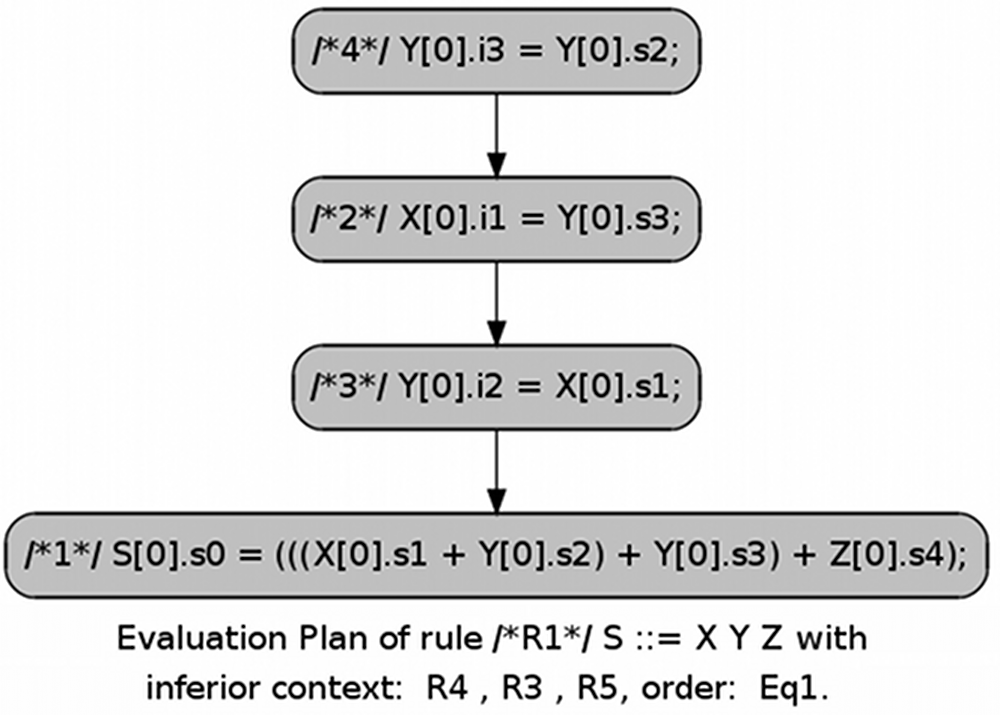
\includegraphics[scale=0.32]{./23_plan_graph.png}
    \end{center}
}

\frame{
  \frametitle{\maggen: Secuencia de visita}

  \begin{block}{}
    \begin{itemize}
      \item Traducción de planes de evaluación a secuencia de visita: \textbtt{compute}, \textbtt{visit}, \textbtt{leave}.
      \item Se basa en la aplicación de un recorrido sobre los planes de evaluación resolviendo las dependencias para evaluar los atributos.
    \end{itemize}
  \end{block}

  \begin{exampleblock}{}
    \begin{tabular}{p{4cm} c p{5cm}}
    Plan de evaluación \textbf{$\{ Eq_{1}, Eq_{2}, \ldots Eq_{n}\}$}& $\Longrightarrow$ & Acciones capaces de moverse sobre un AST; \textbf{\{visit($node_{1}$), compute($Eq_{1}$),$\ldots$,  compute($Eq_{n}$)\}}
    \end{tabular}
  \end{exampleblock}
}

\frame{
  \frametitle{Heurística del algoritmo}
  \begin{enumerate}
    \item Se recorre el plan tomando en cada paso una de las ecuaciones.

    \item Dada la ecuación \textbtt{i}, en el plan, se debe computar todo el \textit{l\_value} de la ecuación. Para ello se deben resolver todas las dependencias dadas por \textit{r\_value}.

    \item Dada una dependencia de la ecuación, primero se chequea si la misma fue computada en algún paso anterior, sino, se analiza:

      \begin{itemize}
	\item \textbf{Símbolo de la parte izquierda de la regla} asociado a un \textbf{atributo heredado}, realizar un ``\textbtt{leave}''.

	\item \textbf{Símbolo de la parte derecha de la regla} y además contiene un \textbf{atributo sintetizado}, realizar un ``\textbtt{visit}''. \textbf{Elección de plan}. 
      \end{itemize}

    \item Luego de la obtención de todas las dependencias, se realiza un \texttt{compute} del \textit{l\_value} y se marca a este como \textbtt{evaluado}.
  \end{enumerate}
}

\begin{frame}[fragile]

\begin{figure}[h]
\begin{center}
\begin{tabular}{c}
\begin{lstlisting}[basicstyle=\scriptsize, language=, linewidth=7.6cm]
(R1) S `$\rightarrow$` XYZ
       (1) S.s0 := X.s1 + Y.s2 + Y.s3 + Z.s4
       (2) X.i1 := Y.s3
       (3) Y.i2 := X.s1
       (4) Y.i3 := Y.s2
...
\end{lstlisting}
\end{tabular}
\end{center}
\end{figure}

    \begin{tabular}{cc}
        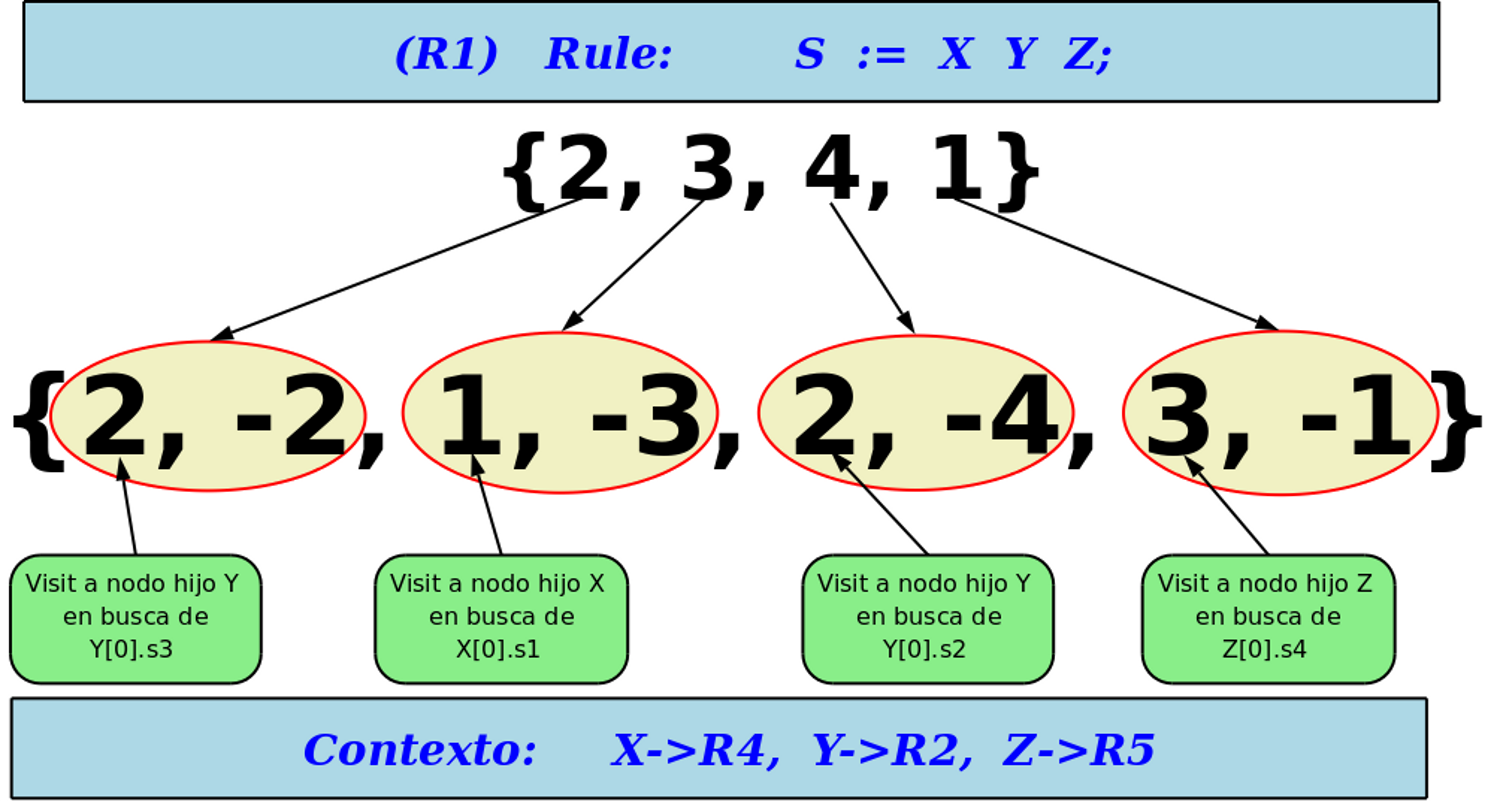
\includegraphics[width=200px, height=107px]{./plan2seq.png}&
        \hspace{0.2cm}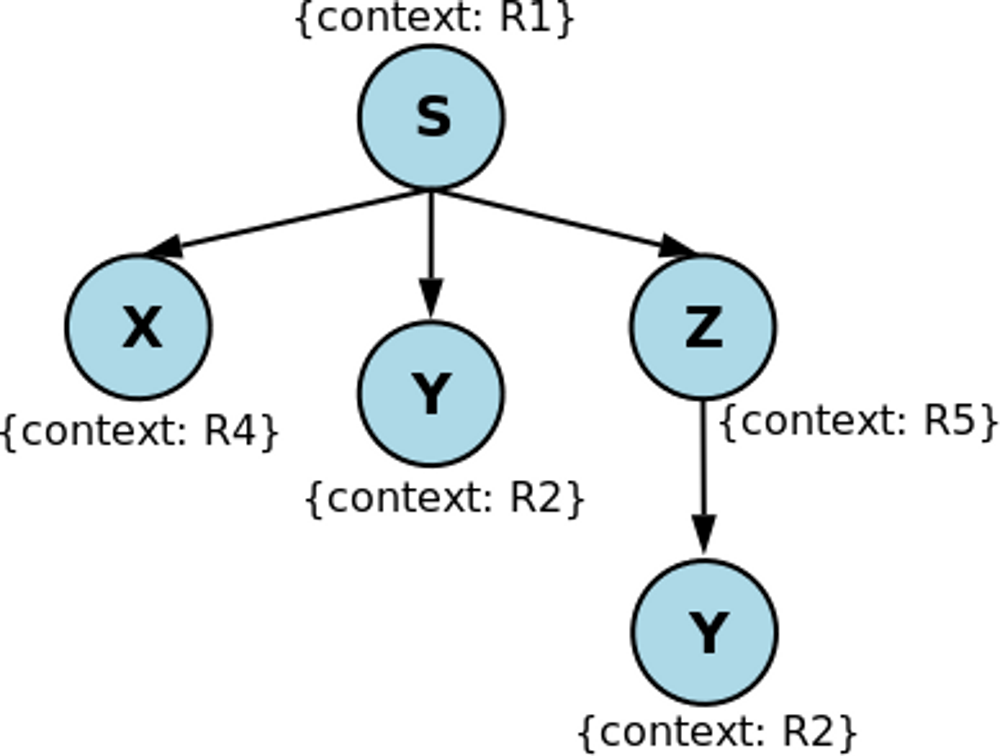
\includegraphics[width=100px, height=76px]{./ast.png}
    \end{tabular}

\end{frame}
\subsection{Generacion de código}

\frame{
    \frametitle{Generación de código}
    
    \begin{block}{}
         La etapa final de \maggen\ esta dada por la generación de código para el evaluador estático. Esta, produce dos archivos: \textit{interface} (.hpp) e \textit{implementación} (.cpp). Los archivos generados se vinculan con dos módulos estáticos, \texttt{Node.hpp} y \texttt{Node.cpp}.
    \end{block}
    
    Los módulos generados contienen:
    
    \begin{itemize}
        \item Los planes de evaluación.
        \item Las secuencias de visita.
        \item Las reglas de la gramatica.
        \item Cada símbolo de la gramatica es implementado mediante \texttt{structs} de C++.
        \item Conjunto de métodos para la evaluación.
    \end{itemize}
}
\frame{
    \frametitle{Algoritmo de evaluación}

    Se basa en dos etapas bien definidas:

    \begin{description}
        \item [Primera recorrida del AST] se invoca a la función
            \begin{itemize}
                \item \textbtt{traverse}: responsable de seleccionar el plan de evaluación para cada nodo no terminal.
            \end{itemize}

        \item [Segunda recorrida del AST] se invoca a la función
            \begin{itemize}
                \item \textbtt{eval\_visiter}: es un evaluador orientado a visitas, que debe computar los valores de los atributos de los nodos.
            \end{itemize}
    \end{description}
}

\frame{
    \frametitle{Usando \maggen}
    \begin{block}{}
     Luego de la instalacion, \maggen\ puede ser invocado desde la linea de comandos.
    \end{block}

    \begin{exampleblock}{Argumentos de \maggen}
        \begin{description}
            \item [\textbtt{-f  file}] Entrada de \maggen\ como \textbtt{file}. Por defecto, (\textbtt{cin}) hasta \textbtt{EOF} (End Of File).

            \item [\textbtt{-i  header}] Incluir \textbtt{header} en la generación de código.

            \item [\textbtt{-fo folder}] Directorio de salida para \maggen. Por defecto ``\textit{./out\_maggen/}''.

            \item [\textbtt{-o  name}] Define a \textbtt{name} como el nombre de la clase y del archivo generado por \maggen. Por defecto el nombre ``\textbf{mag\_eval}''.

            \item [\textbtt{-h}] Muestra mensaje de ayuda.
        \end{description}
    \end{exampleblock}
}

\frame{
    \underline{Ejemplo}: {\scriptsize\textbtt{./maggen -fo ./out\_wuu\_yang -o evalmag -f ./examples/ag\_wuu\_yang/ag\_wuu\_yang.input}}
}

\section{Evaluador generado}

\frame{
    \frametitle{Evaluador generado}
    
    Para el uso del evaluador generado por \maggen\ se necesitan los 4 archivos generados en el directorio de salida:
    
    \begin{itemize}
        \item \textbtt{maggen.hpp}.
        \item \textbtt{maggen.cpp}.
        \item \textbtt{Plan.hpp}.
        \item \textbtt{Node.hpp}.
    \end{itemize}
    
    \begin{exampleblock}{}
        \begin{center}
            AST \hspace{1cm} $\Longrightarrow$ \hspace{1cm} \maggen \hspace{1cm} $\Longrightarrow$ \hspace{1cm} AST decorado.
        \end{center}
    \end{exampleblock}
}

\begin{frame}[fragile]
    \frametitle{Construcción de AST de entrada}

\begin{lstlisting}[columns=fullflexible, basicstyle=\scriptsize, language=c++]
...     
    `\textbf{maggen eval\_mag;}`
    `\textbf{S node\_s1({\color{red}1});}`
    `\textbf{X node\_s1\_x({\color{red}4});}`
    `\textbf{Y node\_s1\_y2({\color{red}2});}`
    `\textbf{Z node\_s1\_z({\color{red}5});}`
    `\textbf{Y node\_s1\_z\_y3({\color{red}2});}`
    `\color{red}\textbf{node\_s1.add(\&node\_s1\_x).add(\&node\_s1\_y2).add(\&(node\_s1\_z.add(\&node\_s1\_z\_y3)));}`
    `\color{blue}\textbf{eval\_mag.evaluator\_mag(\&node\_s1);}`
    cout << " After evaluation." << endl;
    cout << node_s1.to_string() << endl;
...
\end{lstlisting}

    \begin{center}
        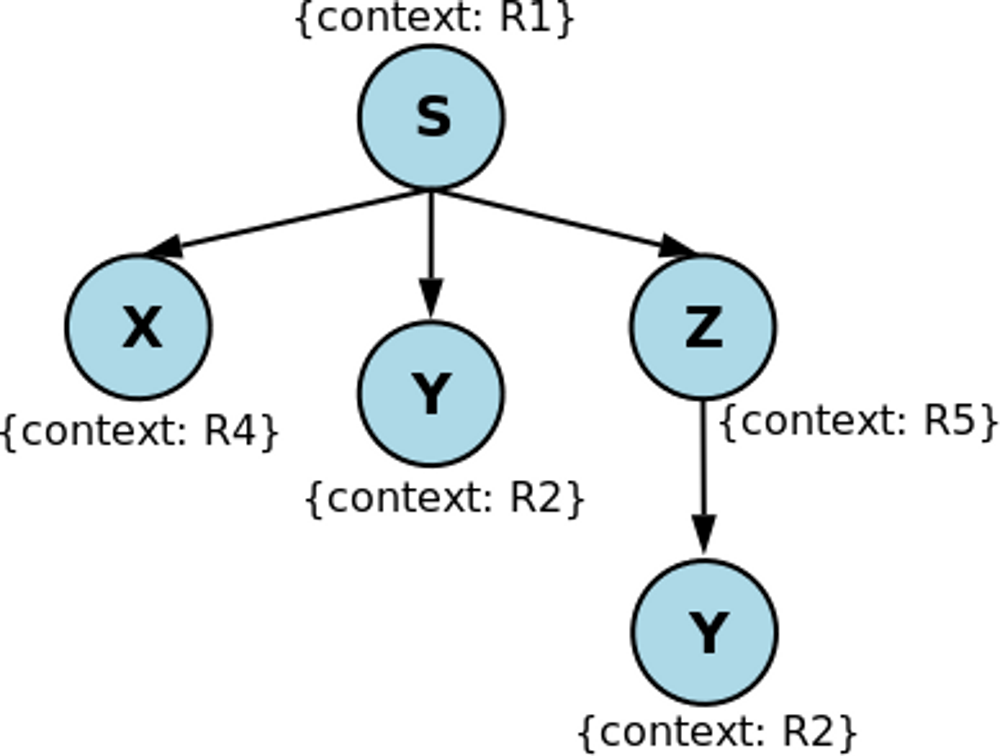
\includegraphics[width=100px, height=76px]{./ast.png}
    \end{center}

\end{frame}


%\frame{
%    \frametitle{magGen - Secuencia de visita}
    
%   \begin{block}{Secuencia de visita generada para el plan\\ R1 $\rightarrow$ R2 R3 R4}
%	    \begin{center}
%	        \vspace{0.1cm}
%	        \textbf{Visit R2 $\Rightarrow$\\
%	        \vspace{0.1cm}
%	        Compute X[0].i1 $\Rightarrow$\\
%	        \vspace{0.1cm}
%	        Visit R4 $\Rightarrow$\\
%	        \vspace{0.1cm}
%	        Compute Y[0].i2 $\Rightarrow$\\
%	        \vspace{0.1cm}
%	        Visit R2 $\Rightarrow$\\
%	        \vspace{0.1cm}
%	        Compute Y[0].i3 $\Rightarrow$\\
%	        \vspace{0.1cm}
%	        Visit R5 $\Rightarrow$\\
%	        \vspace{0.1cm}
%	        Compute S[0].s1} 
%	    \end{center}
%    \end{block}
%}

%\frame{
%    \frametitle{magGen}
%
%    \begin{block}{Informaci\'on de input del evaluador}
%	    \'Arboles Atribuidos representados con AST\footnote{Attribute Syntax Tree}.
%    \end{block}
%    \pause

%    \begin{block}{Informaci\'on de output del evaluador}
%	    El AST decorado\footnote{Cada uno de sus atributos se encuentran calculados}.
%    \end{block}
%}

%\frame{
%    \frametitle{magGen}

%    \begin{block}{Objetivo Subyacente}
%	    Implementar Lenguajes de Propósitos Específicos para problemas puntuales.
%    \end{block}
%}

%\subsection{Detalles de implementación}

\frame {
    \frametitle{Detalles de implementación}

    \begin{block}{}
	    bla bla
    \end{block}
}


%\subsection{Evaluador generado}

\frame {
    \frametitle{Evaluador generado}

    \begin{block}{}
	    bla bla
    \end{block}
}

\section{Performance}
\frame{
    \frametitle{Medidas de performance: Unicidad de planes}

    En un principio cada plan contenía el contexto y la lista de ecuaciones que lo definían. Esto llevo a una \textbf{saturación en la cantidad de planes}.

    \begin{exampleblock}{}
        En la mayoria de los casos la explosión de planes se producía por la cantidad de contextos: \textbf{Planes repetidos}
    \end{exampleblock}

    \begin{block}{}
        \begin{itemize}
            \item La unicidad de los planes permitió una \textbf{reducción notable} en la cantidad de planes.
            \item Optimización destacable en la generación de código del evaluador.
        \end{itemize}
    \end{block}
}

\frame{
    \frametitle{Medidas de performance: Unicidad de planes (cont.)}

   \begin{block}{Ejemplo Aritmetica de expresiones}
        \begin{figure}[h]
        \begin{center}
        \setlength{\doublerulesep}{0mm}
        \setlength{\arrayrulewidth}{0.9pt}
        \begin{tabular}{|l||c|c|}
            \hline
            \rowcolor{gris} \textbf{Variable/Unicidad}&\textbf{Sin} & \textbf{Con} \\ \hline
            \rowcolor{white}\textbf{Cant. de planes}           & 371                        & 371                         \\ \hline
            \rowcolor{white}\textbf{Cant. de planes proy.}     & 687                        & 687                         \\ \hline
            \rowcolor{white}\textbf{Cant. de sec. de visita }  & \color{red}371             & \color{blue}22              \\ \hline
            \rowcolor{white}\textbf{Generación del evaluador}  & \color{red} $\sim$1.44 sec & \color{blue} $\sim$0.47 sec \\ \hline
			\rowcolor{white}\textbf{Cant. de líneas (eval.)}   & \color{red}17464           & \color{blue}5974            \\ \hline
        \end{tabular}
        \end{center}
        \end{figure}
   \end{block}
}

\frame{
    \frametitle{Medidas de performance: Versión de Boost}

    \begin{block}{}
        {\footnotesize
        \underline{\textbf{Computadora}}: Microprocesador Intel Core 2 Duo T5550 1.83 GHz, 2 MB memoria caché L2, 3 GB memoria RAM a 667 MHz.\\
        \underline{\textbf{Sistema operativo}}: GNU/Linux Ubuntu 10.04, Kernel 2.6.32-23, GNU g++ 4.4.3.}
    \end{block}

    \begin{block}{Tiempos de generación de evaluadores de \maggen}
        \begin{figure}[h]
        \begin{center}
        \setlength{\doublerulesep}{0mm}
        \setlength{\arrayrulewidth}{0.9pt}
        \begin{tabular}{|l||c|c|}
            \hline
            \rowcolor{gris} Input / Spirit           & \textbf{1.8.X}   & \textbf{2.3}    \\ \hline
            \rowcolor{white}\textbtt{MAG Wuu Yang}   & $\sim$0.087 sec & $\sim$0.084 sec \\ \hline
            \rowcolor{white}\textbtt{MAG Aritmetica} & $\sim$0.590 sec & $\sim$0.470 sec \\ \hline
        \end{tabular}
        \end{center}
        \end{figure}
    \end{block}
}

\frame{
    \frametitle{Medidas de performance: Compilación evaluador}

    \begin{block}{Tiempos de compilación del evaluador generado}
        \begin{figure}[h]
        \begin{center}
        \setlength{\doublerulesep}{0mm}
        \setlength{\arrayrulewidth}{0.9pt}
        \begin{tabular}{|l||c|c|}
            \hline
            \rowcolor{gris} Input / g++          & \textbf{sin -O3} & \textbf{con -O3}             \\ \hline
            \rowcolor{white}\textbtt{Wuu Yang}   & $\sim$1.51 sec   & $\sim$2.55 sec               \\ \hline
            \rowcolor{white}\textbtt{Aritmetica} & $\sim$5.98 sec   & \textbf{$\sim$1 min 5.6 sec} \\ \hline
        \end{tabular}
        \end{center}
        \end{figure}
    \end{block}

    \begin{block}{Tamaños del ejecutable del evaluador generado}
        \begin{figure}[h]
        \begin{center}
        \setlength{\doublerulesep}{0mm}
        \setlength{\arrayrulewidth}{0.9pt}      
        \begin{tabular}{|l||c|c|}
            \hline
            \rowcolor{gris} Input / g++          & \textbf{sin -O3} & \textbf{con -O3} \\ \hline
            \rowcolor{white}\textbtt{Wuu Yang}   & 104 Kb           & \ 48 Kb          \\ \hline
            \rowcolor{white}\textbtt{Aritmetica} & 516 Kb           & 384 Kb           \\ \hline
        \end{tabular}
        \end{center}
        \end{figure}
    \end{block}
}

\section{Comentarios Finales}

\frame{
    \frametitle{Trabajos Futuros}

    \begin{itemize}
	    \item Implementar la generación de código al estilo ``\textit{plugins}''. Lo que permitiría extensiones varias, transparentes y elegantes para generar código en diferentes lenguajes. Esto implicaría la definición de una API del motor de generación de código.
	    \pause

	    \item Definir una API para la construcción de los AST de entrada al evaluador generado, lo que permitiría que herramientas externas puedan generar los AST entrada.
	    % Este puntos podría ser analizado teniendo en cuenta los A-Terms como ejemplo.
	    \pause

	    \item Pruebas de rendimiento como comparaciones con otras herramientas similares.
	    % (Silver, definir sintaxis y semántica, es modular, puede que genere evaluador dinámico)
	    \pause

	    \item Permitir definir atributos de \textbf{alto orden}, es decir, atributos que pueden ser un árbol. Para los cuales, su evaluación supondría un nuevo proceso de igual complejidad que el necesario para decorar al AST de entrada.
	    \pause

	    \item Implementar como especies de templates para los atributos.
    \end{itemize}
}

\frame{
    \frametitle{Extensiones}

    \begin{itemize}
	    \item Extensiones al lenguaje de especificación, como módulos a través de \texttt{\#include}. Esto engloba los puntos siguientes:

	        \begin{itemize}
		        \item Disponer de espacios de nombres, y operadores que permitan referirse a estos \textbf{espacios de nombres}.

		        \item Redefinición o extensión de reglas incluidas, un estilo de \textbf{sobrecarga}.

		        \item Permitir el \textbf{adicionado de atributos} a símbolos pertenecientes a otros módulos.
	        \end{itemize}
    \end{itemize}
}


\frame {
    \begin{block}{}
	    bla bla
    \end{block}
}

\section{Bibliografía}
    \frame{
	\frametitle{Bibliografía}\scriptsize

	\begin{thebibliography}{66}
	    \bibitem {wuu-yang1} Wuu Yang. 1998. \textit{Multi-Plan Attribute Grammars}. Department of Computer Information Science. National Chiao-Tung University, Hsin-Chu, Taiwan.

	    \bibitem {wuu-yang2} Wuu Yang. 1999. \textit{A Classification of Non Circular Attribute Grammars based on Lookahead behavior}. Department of Computer and Information Science. National Chiao-Tung University, Hsin-Chu, Taiwan.

	    \bibitem {wuu-yang3} Wuu Yang. 1998. \textit{Conditional Evaluation in Simple Multi-Visit Attribute Grammar Evaluators}. Department of Computer and Information Science. National
	    Chiao-Tung University, Hsin-Chu, Taiwan.

	    %\bibitem{wuu-yang4} Wuu Yang, W. C. Cheng. \emph{A Polynomial Time Extension to Ordered Attribute Grammars}. Department of Computer and Information Science.National Chiao-Tung University, Hsin-Chu, Taiwan.

	    %\bibitem {gramática} John E. Hopcroft, Rajeev Montwani, Jefrey D. Ullman.\textit{Introduction to Automata theory, languajes, and computation}. Addison-Wesley (2001) second edition.

	    \bibitem {compiladores} Alfred V. Aho, Ravi Sethi, Jeffrey D. ullman.\textit{Compilers: Principles, Techniques and Tools}. Addison-Wesley (1985)  Iberoamericana, S.A. Wilmington, Delaware, E.U.A.

	    \bibitem {tesismarcelo} Arroyo, Marcelo Daniel. \textit{Gramáticas de atributos, clasificación y aportes en técnicas de evaluación}. Tesis de carrera de Magíster en Ciencias de la Computación. Universidad Nacional del Sur. Bahía Blanca - Argentina.

	    \bibitem {kastens} U. Kastens. 1980. \textit{Ordered Attribute Grammars}. Acta Informática. Vol. 13, pp. 229-256.

	    \bibitem{intri-exc} Jazayeri, Ogden and Rounds. 1975. \emph{The intrinsically exponential complexity of the circularity problem for attribute grammars}. Comm. ACM 18. December 2, Pag: 697-706.
	\end{thebibliography}
    }

    \frame{
	\frametitle{Bibliografía (Cont.)}
    \scriptsize
	\begin{thebibliography}{66}
	    %\bibitem {meyer} Bertrand, Meyer (1997). \textit{Object-Oriented Software Construction}. Segunda edición. Prentice Hall Professional Technical Reference. Santa Barbara (California).

	    %\bibitem {estruc-algorit} Alfred V. Aho, John E. Hopcroft, Jefrey D. Ullman. \textit{Data Structures and Algorithms}. Addison-Wesley publishing Company, Reading, Massachusetts, E. U. A.(1983).

	    %\bibitem {valen} Valentin David. \textit{Attribute Grammars for C++ Disambiguation}. LRDE, 2004.

	    \bibitem {Knuth} D. Knuth. 1968. \textit{Semantics of context free languages}. Math Systems Theory 2.June 2.Pag: 127-145.

	    %\bibitem {eclipse} \textbf{eclipse}. \textit{Multi-language software development environment.} URL:\urllink{http://www.eclipse.org/}.
	    
	    %\bibitem {doxy} \textbf{doxygen}. \textit{A documentation generator for C++, C, Java, Objective-C, Python, IDL (CORBA and Microsoft flavors), Fortran, VHDL, PHP and C\#}. URL: \urllink{www.doxygen.org}.

	    \bibitem{c++1} \textbf{C++}. \textit{C++ Annotations Version 8.2.0.} URL: \urllink{http://www.icce.rug.nl/documents/cplusplus/}. 

	    \bibitem{c++2} \textbf{C++}. \textit{C++ reference} URL: \urllink{http://www.cppreference.com/wiki/es/start}. 

	    \bibitem{latex} \textbf{\LaTeX}. \textit{A document preparation system} URL: \urllink{http://www.latex-project.org/}.

	    \bibitem{boost} \textbf{Boost}. \textit{Boost C++ Libraries}. URL: \urllink{http://www.boost.org/}.
	\end{thebibliography}
    }

\end{document}
